\documentclass[conference]{IEEEtran}
\IEEEoverridecommandlockouts
% The preceding line is only needed to identify funding in the first footnote. If that is unneeded, please comment it out.
\usepackage{cite}
\usepackage{amsmath,amssymb,amsfonts}
\usepackage{algorithmic}
\usepackage{graphicx}
\usepackage{textcomp}
\usepackage[table]{xcolor}

\def\BibTeX{{\rm B\kern-.05em{\sc i\kern-.025em b}\kern-.08em
    T\kern-.1667em\lower.7ex\hbox{E}\kern-.125emX}}
\begin{document}

\title{Consumer Price Index Analysis and Forecasting}

\author{\IEEEauthorblockN{Pedro sá}
\IEEEauthorblockA{\textit{University of Coimbra}\\
Coimbra, Portugal \\
pedronuno@student.dei.uc.pt}
\and
\IEEEauthorblockN{Alexandre Santos}
\IEEEauthorblockA{\textit{University of Coimbra}\\
Coimbra, Portugal \\
alexandresantos@student.dei.uc.pt}
}

\maketitle

\begin{abstract}
The Consumer Price Index (CPI) is a macroeconomic indicator that measures price changes for goods and services purchased by households to meet a set of desires and requirements, and is commonly leveraged by governments for estimating inflation and policy-making. A proper modelling of the CPI can be key for better decision-making on the economic state of a country. In this paper, we comprehensively analyze and forecast Denmark's CPI. 
\end{abstract}

\begin{IEEEkeywords}
time series, forecasting
\end{IEEEkeywords}

\section{Introduction}
The Consumer Price Index (CPI) is a macroeconomic metric of the price changes for goods and services acquired by households to satisfy a set of wants and needs. This index is important for decision-making processes in governments and institutions, e.g., for providing precise estimates of inflation, and thus poses a handy reflection of the general economic state and well-being of a country.

An accurate modelling of a country's CPI is key to understanding out it behaves now, and how it will behave in the future. Moreover, it's unquestionably useful for predicting periods of inflation, allowing governments to better handle market dynamics before they happen.

In this paper, we present a case study on the country of Denmark, comprising an analysis and forecasting model of the CPI.

\subsection{Related Work}
\subsection{Data}
In order to perform such study, a dataset consisting of CPI (and several other indicators) records was made available. From the 191 available countries, we selected Denmark as a subject of study and therefore extracted a time series of monthly CPI (all items) values from 1990 up until 2022.

\begin{figure}[hbtp]
    \centering
    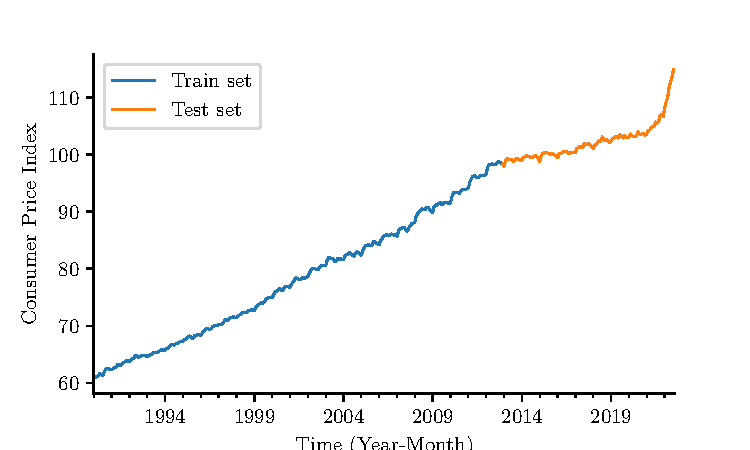
\includegraphics{../figs/cpi.pdf}
    \caption{Denmark CPI (All Items)}
    \label{fig:cpi}
\end{figure}

The time series was split into a training and test set in a $70/30$ ratio, respectively. Figure \ref{fig:cpi} illustrates the evolution of the CPI over a span of 22 years for the country of Denmark.

\section{Methods}
The following section describes in detail the methods used for characterization, modelling and forecasting of the time series.
\subsection{Characterization}
Preliminary observations suggest that the time series better fits a multiplicative model of the form:
\[
ts(n)=tr(n)\cdot sn(n)\cdot \epsilon(n)
\]

given the seeming independence of the seasonality and erratic component from the "apparent" trend.
\subsubsection{Trend}
The trend component was described by three different techniques. \textbf{Polynomial fitting} is the process of fitting a polynomial curve of order $n$
\[
tr(n) = \beta _0+\beta_ 1n+\beta_ 2n^2\dotsb+\beta _kn^k
\]

for which the coefficients $\lbrace\beta_i\rbrace^k_{i=1}$ are estimated by minimizing a $l_2$ cost function
\[
\min\,\sum\Bigl(x(n)-tr(n)\Bigr)^2
\]

with respect to the residuals. Linear and Quadratic fitting were used in this paper.

\textbf{Moving-Average} is a local smoothing technique that averages the values on a \textit{moving} time window $M$ along the timeseries,
\[
\hat{tr}(n)=\frac{1}{\sum w_k}\sum^{n+\frac{M-1}{2}}_{n-\frac{M-1}{2}} \omega_kx(n+k)
\]

thus removing some randomness from the data. The moving average implements data augmentation to account for the non existent samples, at the beginning and at the end of timeseries, needed to calculate the average.

\textbf{LOcally WEighted Scatterplot Smoothing (LOWESS)} is a non-parametric approach that performs a local weighted regression over the $M$ closest points to each data point $(x_i,y_i)$. First, the regression is fit by a weighted $l_2$ cost function, giving more weight to nearby data points. In order to decrease the effect of outliers, further regressions can be performed. In the experimental setup we chose to perform only 1 additional regression.

\textbf{N-order differencing} is a technique for \textit{implicitly} turning non-stationary time series into stationary, by calculating the changes between consecutive observations. The first difference is given by
\[
\acute{ts}(n) = ts(n) - ts(n-1) 
\]

and allows to remove the trend-cycle. Seasonal differencing is of the form
\[
\acute{ts}(n) = ts(n) - ts(n-m)
\]

in which $m$ is the frequency of a seasonal pattern. The latter is used to remove any trace of seasonality and attain stationarity if the first-order difference was not enough.

\subsubsection{Seasonality}
Besides the above mentioned \textbf{n-order differencing}, there are additional techniques to assess seasonality. \textbf{Spectral Analysis} is a technique for finding underlying periodicity in stochastic processes; by transforming a time series from the time domain to the frequency domain, we can characterize it on the basis of its distinct frequencies -- seasonal patterns. The frequency spectrum is calculated by the \textbf{Discrete Fourier Transform}, a technique that decomposes a complex signal in more simple ones, which will yielded the different frequencies -- seasonal patterns -- and corresponding magnitudes.

\textbf{Filtering} builds on top of spectral analysis, because upon isolating the cycles, these can be removed by filtering the frequencies (or seasonal patterns) of smaller magnitude as to provide a more accurate estimate of the cyclic behaviour. The filter used in this paper is the Butterworth.

\subsubsection{Stationarity}
Along with \textbf{n-order differencing}, stationarity can also be assessed via other methods. \textbf{Autocorrelation analysis} consists of computing the correlation $r_{XX}$ between observations at different time lags, for which $|r_{XX}|>0$ indicates some correlation and $r_{XX}=0$ indicates an absence of correlation. By establishing confidence bounds, considering a significance level of $95\%$, we can say that the autocorrelation is bounded by
\[
-\frac{1.96}{\sqrt{N}}\leq r_{XX}\leq\frac{1.96}{\sqrt{N}}
\]

where values that fall outside this region are \textit{significantly} different from zero and indicate a substantial correlation. For a non-stationary time series, the following is verified
\[
\lim_{T\to\infty}r_{XX}=0
\]

whereas if the autocorrelation quickly drops to zero, it generally means that the time series is stationary. The \textbf{Augmented Dickey-Fuller test} is a statistical test that tests the null hypotheses $H_0$ that a unit root is present in a time series. A time series is considered to be non stationary if a unit root is present and stationary otherwise.

\subsection{Modelling}
For the modelling, considering the time series is indeed non-stationary and exhibits cyclic behaviour, we use a SARIMA model. A SARIMA model extends the ARIMA model with seasonal terms:
\[
    \text{SARIMA}(p,d,q)\text{X}(P,D,Q)_S
\]

where $d$ and $D$ stand for the order of first and seasonal differencing, respectively; $p$ and $P$ represent the Autoregressive (AR) model orders for the non-seasonal and seasonal part of the model, respectively; $q$ and $Q$ stand for the Moving Average (MA) model orders for the non-seasonal and seasonal part of the model, respectively, and $S$ represents the dominant cyclic behaviour.

\subsection{Forecasting}

\section{Results}

\begin{table}[btp]
    \caption{Trend assessment methods}
    \centering
    \begin{tabular}{l|c|c}
         Method & Parameters & MSE \\
         \hline
         Linear & -- &  $1.38\text{e}-04$ \\
         Quadratic & -- & $4.34\text{e}-05$ \\
         Moving Average & $M=13$ & $1.39\text{e}-05$ \\
         LOWESS & $M=13$ & \cellcolor{green!25}$9.43\text{e}-06$ \\
    \end{tabular}
    \label{tab:trend}
\end{table}

\begin{figure}[hbtp]
    \centering
    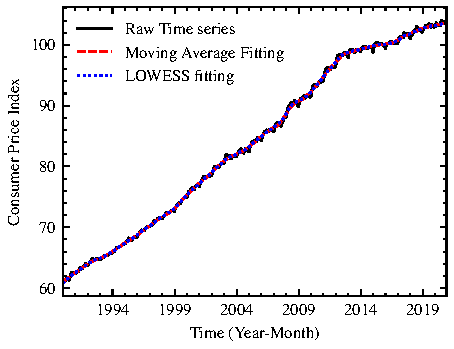
\includegraphics{../figs/trend.pdf}
    \caption{Trend fitting}
    \label{fig:trend}
\end{figure}

The results suggest that the time series's trend is better described by the LOWESS approach as seen in Table \ref{fig:trend} and Figure \ref{fig:trend}. The linear and quadratic trends, due to their low-order nature and usage of the global structure of the data, are not sensitive to oscillations and thus are only able to give a rough approximation. The Moving Average and LOWESS fittings, on the other hand, rely on the local structure of the data and are globally non-linear, allowing them to tend to these oscillations. LOWESS yields a better approximation as it performs multiple local (weighted) regression instead of averages, thus being more sensitive to outliers.

\begin{figure*}[hbtp]
    \centering
    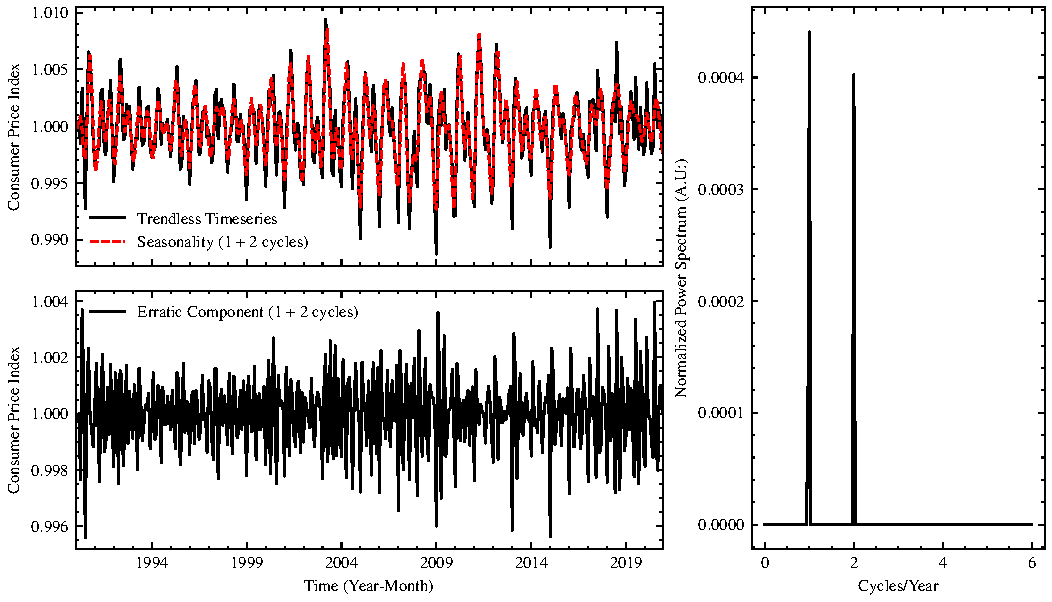
\includegraphics{../figs/season.pdf}
    \caption{The frequency spectrum (right), the trendless timeseries and the seasonality fitting (top left), the estimate erratic component (bottom left).}
    \label{fig:season}
\end{figure*}


Regarding seasonality, a careful glance suggests a clear pattern every 6 months and, less noticeably, every year. Through spectral analysis, we we're able to identify 1 and 2 cycles per year, as seen in Fig \ref{fig:season}, and thus we filtered the other non relevant frequencies. The estimated seasonality is also illustrated in Fig \ref{fig:season}, from which we can observe an adequate estimation of the cyclic behaviour, given that it models both cycles fairly well. Additionally, the erratic component resembles some stationarity, although some patterns still remain visible; this most likely stems from this method relying in estimations and decomposition models.

\begin{figure}[hbtp]
    \centering
    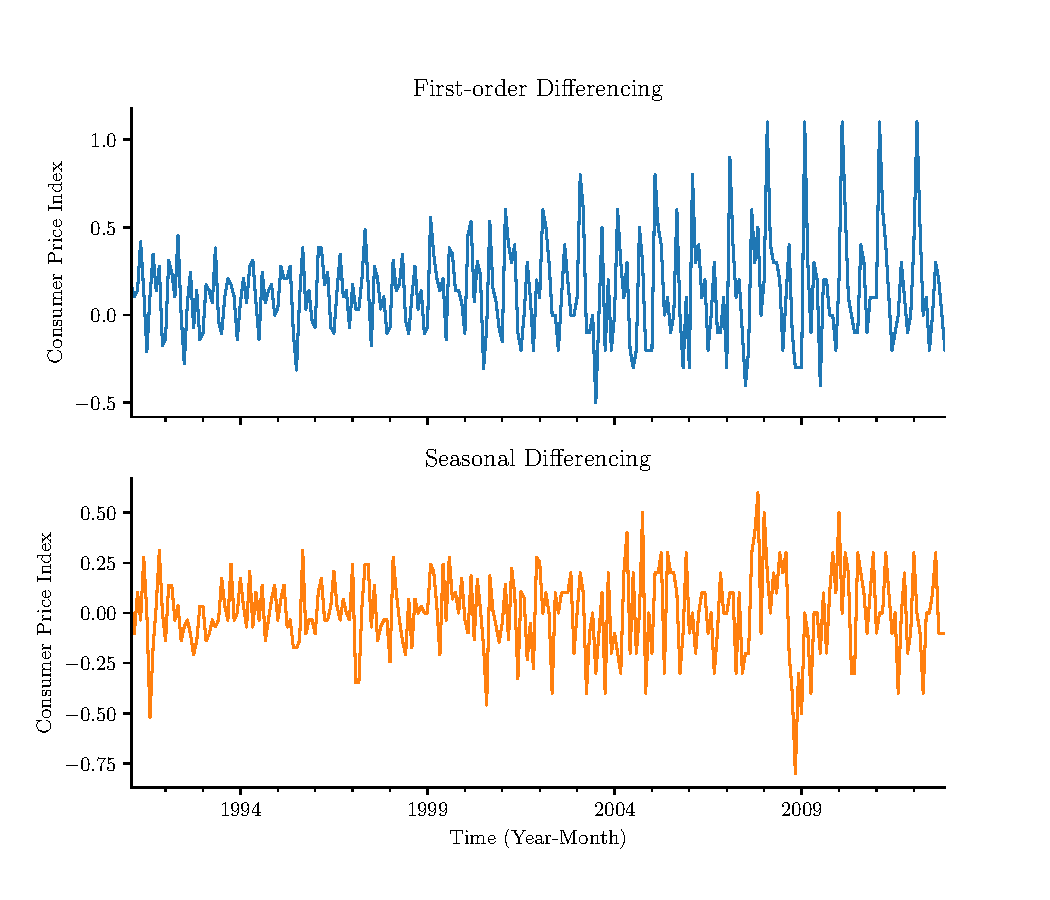
\includegraphics{../figs/differencing.pdf}
    \caption{Stationarity by differencing}
    \label{fig:differencing}
\end{figure}

\begin{figure}[hbtp]
    \centering
    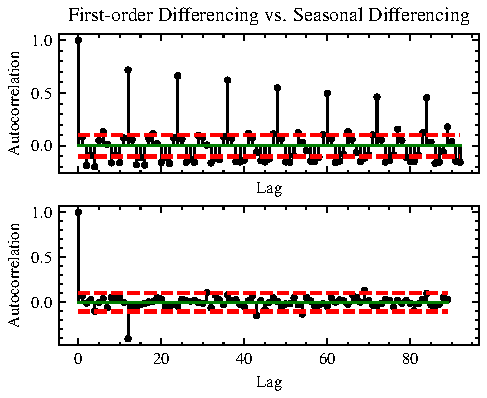
\includegraphics{../figs/acs_diff.pdf}
    \caption{Correlogram of first-order differencing (top) and seasonal differencing (bottom)}
    \label{fig:acs_diff}
\end{figure}

The differencing approach on the other hand, yielded more clarifying results. This may be due to differencing not resorting to the estimation of each individual component, and instead computing the differences between data points and removing the changes in level. As seen in Figure \ref{fig:differencing}, the first difference was not enough to achieve stationarity given some clear patterns and a slight upwards slope, whereas the seasonal difference time series has constant variance and is arguably horizontal. Observing the correlogram in Fig \ref{fig:acs_diff}, we can argue for non-stationarity of the first difference, considering i) most values fall outside of the confidence bounds ii) a strong decreasing autocorrelation for lag values multiple of 6 and 12, which happens to be the most relevant seasonal patterns in the timeseries. On the other hand, the seasonal difference is clearly stationary, given that i) almost all values tend to be within the confidence bounds, apart from a few exceptions\footnote{Probably due to computational errors given the small sample size $N$} ii) the autocorrelation instantly drops to zero.

\begin{table}[btp]
    \caption{ADF test results}
    \centering
    \begin{tabular}{l|c|c||c}
        Subject & \textit{p}-value & ADF Statistic & 1\% Treshold  \\
        \hline
        Raw timeseries & $0.9987$  &  $2.0048$ & $-3.456$ \\
        First difference & \cellcolor{green!25} $0.0087$ & $-3.4741$ & $-3.456$ \\
        Seasonal difference & \cellcolor{green!25} $\approx 0$ & $-7.1215$ & $-3.457$ \\
    \end{tabular}
    \label{tab:adfuller}
\end{table}

Table \ref{tab:adfuller} presents the results of the ADF unit root test. As expected, $H_0$ is accepted for the raw time series, as $p\text{-value}>0.05$, whereas it's actually rejected for the first and seasonal differences, considering the \textit{p}-value is (quite) inferior to $0.05$ and that the test statistic is below the $1\%$ confidence level. While this poses a contradiction for the first difference, one should take into account that the ADF test actually tests if there is or isn't a need for further differencing, thus suggesting that the first difference doens't require any more differencing, which can be construed as stationarity.

\begin{table}[btp]
    \caption{SARIMA grid-search}
    \centering
    \begin{tabular}{c|c|c}
        Parameter & Range & Best \\
        \hline
        $p$ & $[0,2[$ & $1$ \\
        $q$ & $[0,2[$ & $0$ \\
        $P$ & $[0,4[$ & $0$ \\
        $Q$ & $[0,3[$ & $1$ \\
        \hline
        \textbf{Best AIC}& \multicolumn{2}{c}{$\approx -209.7$} \\
        \textbf{Best $\mathcal{L}$}& \multicolumn{2}{c}{$\approx 107.9$} \\
        \textbf{Q-statistic}& \multicolumn{2}{c}{$\approx 0$}
    \end{tabular}
    \label{tab:grid-search}
\end{table}


These kind of assesments allow us to derive the parameters for time series modelling. Because stationary was only attained with a first difference and a seasonal difference, we can set $(d=1;D=1;S=12)$. Moreover, from the ACF and PACF we can guess the AR and MA parameters of the model. Instead, we opted by a grid-search approach for finding the parameters, considering the ACF and PACF are often times deceiving, as the parameters we derived from a visual analysis yielded a higher AIC score ($\approx -204.2$).

% plot the char roots

Figure \ref{} illustrates the characteristic roots for the model fitted to the time series. Both the AR and MA polynomial roots happen to lie outside the unit circle, which is mandatory for preserving the stationarity and invertibility properties of the model. However, the MA roots lie too close to the unit circle: these can become numerically unstable and eventually lead to poor forecasts, as we later discuss.

% plot the train set vs model fitting, residuals and ACF of residuals

Analyzing the residuals provides a clearer picture. The residuals plotting indicates the presence of an i.i.d. process, also considering $\mu_\epsilon\approx -0.0046$. However, the standard deviation is slightly but significantly larger then $\frac{1}{\sqrt{N}}$ ($\sigma_\epsilon\approx 0.17$), which suggest a lot of variance in the residuals. Moreover, given the absence of correlation in the ACF of the residuals (after $T>0$ the values quickly drop to $0$), we can argue the model is adequate.

% Maybe mention Q-statistic

% plot residual distribution

The Figure \ref{} describes the residuals' ACF values distribution, which seems slightly skewed to the left, possibly alerting for non-normally distributed ACF values. Moreover, it seems that the number of available samples has relaxed the confidence bounds to a broader spectrum. It so happens to be that the available data for training consists of only $N=312$ samples, which, and according to the Law of Large Numbers, doesn't provide enough statistical significance for the model to approximate fittings close the expected value. Such is also evident by the close, but not quite right, approximation to the theoretical probability density function. Some experiments revelead that, by reserving more data to the training (and less for testing), we were able to achieve optimal results, although at the expense of not enought data for forecasting.

\section{Discussion}

%\bibliography{bib}
%\bibliographystyle{plain}

\end{document}
